% !TEX root = ../thesis.tex

%In this thesis we consider sampling or approximating distributions that factorise in a specific way. 
In this chapter, we cover the Local Bouncy Particle Sampler (LBPS), a version of the BPS introduced in chapter \ref{chap:BGsampling}, section \ref{point:BPS} for target distributions that factorise according to a MRF.

The aim of this short chapter is to show that the LBPS algorithm can be used on high-dimensional models such as probabilistic matrix factorisation and performances are not far those of the HMC algorithm thereby showing the potential of PDMP samplers on complex Machine Learning models. For this, we used our open-source package \texttt{PDSampler.jl} coded in Julia.\footnote{\url{https://github.com/alan-turing-institute/PDSampler.jl}} 

\section{Local Bouncy Particle Sampler}
In \cite{bouchard15}, the authors consider the case where the target distribution factorises as
%
\eqa{
	\pi(x)&\propto& \prod_{f\in F} \gamma_{f}(x_{f})
}
%
where $x_{f}$ is a restriction to a few elements of $x$, $F$ is a set of \emph{factors} and $\gamma_{f}$ is an unnormalised likelihood associated with the factor. In the specific case of a pairwise MRF, the factors are the edges of the graph and the restrictions are the variables corresponding to each nodes. The energy associated to $\pi$ consequently decomposes as $U\equiv \sum_{f\in F}U_{f}$.

%\subsection{Local BPS: algorithm}
For each factor, a local intensity $\lambda_{f}$ and a local bouncing operator $R_{f}$ can be defined in the same way as for the Bouncy Particle Sampler (BPS, see section \ref{point:BPS}) except that $\nabla U_{f}$ is set to have zero components for all variables not associated with the factor. We can then define a collection of intensities with
%
\eqa{
	\chi_{f}(t) &=& \lambda_{f}(x^{(i-1)}+v^{(i-1)}t,v^{(i-1)}). 
}
%
and consider the superposition principle with $\chi\equiv\sum_{f} \chi_{f}$ (see point \ref{point:BPS}).

Instead of modifying all velocity variables at a bounce as in the basic BPS, the method samples a factor $f$ with probability $\chi_{f}(\tau)/\chi(\tau)$ and modifies only the variables connected to the sampled factor. 
This can significantly reduce the overall computational cost associated with the algorithm and especially so when the underlying MRF has a connection structure that is not too densely connected. Indeed, when an update is triggered at a factor $f$ all factors that share a variable with $f$ are also triggered. If that corresponds to a large portion of the graph, computational gains are lost compared to simply using the full BPS. The skeleton of the algorithm is shown below.



%\subsection{Local BPS Algorithm}
%
\begin{algorithm}[!h]\small
	\caption{\label{alg:LBPS}\small \idblue{Local BPS with Priority Queue}}
	\begin{algorithmic}[1]
	\State initialise $(x^{(0)},v^{(0)})$, set $t_{\text{clock}}=0$
	\State simulate a first arrival time $\tau_{\text{bounce}}^{f}\sim \text{PP}(\chi_{f}(t))$ for each factor $f$
	\State initialise a priority queue $Q$ with the couples $\{(\tau_{f}, f)\}_{f\in F}$
	\State initialise event lists $L_{f}$ for each factor with $(x^{(0)}_{f}, v^{(0)}_{f}, 0)$
	\State sample $\tau_{\text{ref}}\sim\mathrm{Exp}(\lambda_{\text{ref}})$
	\While{more events requested}
		\State pop $(\tau_{f}, f)$ from $Q$ based on the smallest bounce time
		\If{$\tau_{f}>\tau_{\text{ref}}$} 
			\State $t_{\text{clock}}\leftarrow t_{\text{clock}}+\tau_{\text{ref}}$
			\State sample a new $v\sim \mathcal N(0, \mathbb I)$
			\State start a new queue $Q$ where the positions for each factor is extrapolated linearly until the refreshment time
		\Else
			\State $t_{\text{clock}}\leftarrow t_{\text{clock}}+\tau_{f}$
			\State extrapolate $x_{f}$ linearly until $t_{\text{clock}}$
			\State add $x_{f}$ to the list $L_{f}$
			\For{all neighbouring factors $f'$}
				\State extrapolate $x_{f}'$ linearly until $t_{\text{clock}}$
				\State simulate the first arrival time $\tau_{f'}$ of a PP with intensity $\lambda_{f'}(x_{f'}+tv_{f'}, v_{f'})$
				\State update $Q$ with these candidate bounce times
			\EndFor
		\EndIf
	\EndWhile
	\end{algorithmic}
\end{algorithm}



\section{Probabilistic Matrix Factorisation}

Probabilistic Matrix Factorisation (PMF) \citep{mnih08} is a Bayesian approach to the matrix completion problem. In that problem, we consider a matrix $R$ of size $n\times p$ of ratings $r_{ij}$ corresponding to user $i$ and item $j$ (e.g.: a movie) but we only have access to a mask of $R$, a very sparse subset of the ratings which we denote $\hat R$. The aim of matrix completion methods such as PMF is to try to construct a low-rank factorisation  $R\approx U^{t}V$ based on the known entries, where $U$ is of size $d\times n$ and $V$ of size $d\times p$ and $d$ is very small compared to $n$ or $p$. 

\subsection{Description of the  Model}

The model described in \citet{mnih08} assumes that each rating $r_{ij}$ is a realisation from a Normal random variable with mean $\scal{u_{i}, v_{j}}$ and standard deviation $\sigma_{r}$. 
Further, the model assumes spherical Gaussian priors on all $u_{i}$ and $v_{j}$ with standard deviation $\sigma_{u}$ and $\sigma_{v}$ respectively. Formally:
%
\begin{eqnarray}
	r_{ij} &\sim& \mathcal N(\,\cdot\, ; \scal{u_{i}, v_{j}}, \sigma_{r}^{2}), \qquad (i,j)\in\mathcal M\nn\\
	u_{i} &\sim& \mathcal N(\,\cdot\, ; 0_{d}, \sigma_{u}^{2}\mathbb I_{d}), \qquad i\in 1,\dots,n \label{eq:pmf-model}\\
	v_{j} &\sim& \mathcal N(\,\cdot\, ; 0_{d}, \sigma_{v}^{2}\mathbb I_{d}), \qquad j\in 1,\dots,p\nn
\end{eqnarray}
%
where $\mathcal M$ denotes the entries which are available, $0_{d}$ and $\mathbb I_{d}$ denote the zero vector in $\mathbb R^{d}$ and the $d\times d$ identity matrix respectively. 
The negative log-posterior of interest is therefore:
%
\eqa{
- \log p(U, V|\hat R) &=& {1\over 2\sigma_{r}^{2}}\sum_{(i, j)\in\mathcal M} (r_{ij}-\scal{u_{i}, v_{j}})^{2} +
{1\over2\sigma_{u}^{2}}\|U\|_{2}^{2} +
{1\over2\sigma_{v}^{2}}\|V\|_{2}^{2}
}
%
In our experiments, we assume $\sigma_{r}, \sigma_{u}$ and $\sigma_{v}$ are fixed,\footnote{In practice, we compute sensible estimates from the data following the authors' original code available at \url{http://www.cs.toronto.edu/~rsalakhu/BPMF.html}.} more involved models exist including hyper-priors which we will not consider here since our aim is primarily to compare the local BPS and HMC on a large scale model rather than produce the best performing PMF method.\footnote{In \citep{mnih08}, the authors also suggest doing a few steps of Gibbs sampling for the hyperparameters. We do not do this in order to simplify the computations and the comparisons.}

Finally, note that the full dimensionality of the model is $n\times d + p\times d$. Below we consider an example where $d=10$, $n=6000$, $p=4000$ and $|\mathcal M|=10^{6}$ meaning that the full dimensionality of the model is $100 000$ with 1 million factors. For that kind of scale, a method such as naive Gibbs sampling (see point \ref{point:classical-sampling}) is impractical. 


\subsection{Local BPS for the PMF}

The factor graph corresponding to the matrix factorisation problem has a simple structure: each rating $r_{ij}$ for $(i,j)\in\mathcal M$ corresponds to a factor connected to the variables $u_{i}$ and $v_{j}$. This is illustrated in figure \ref{fig:pmf-graph} below.

\begin{figure}[!h]
\center
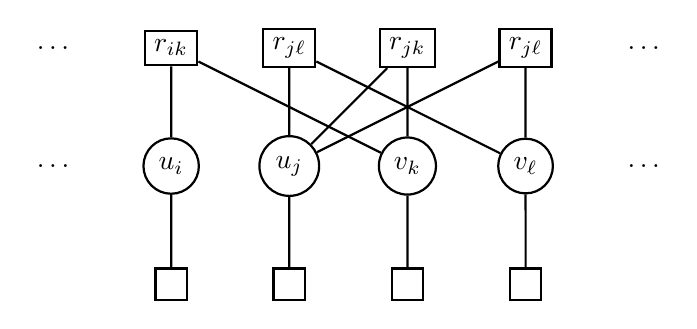
\begin{tikzpicture}[-,minimum size=.4cm,scale=.1,node distance=1.5cm, thick]
	\node[]				(A0)				{$\dots$};
	\node[rectangle,draw]	(A) [right of=A0]	{$r_{ik}$};
	\node[rectangle,draw] 	(B) [right of=A]		{$r_{j\ell}$};
	\node[rectangle,draw]	(C) [right of=B]		{$r_{jk}$};
	\node[rectangle,draw]	(E) [right of=C]		{$r_{j\ell}$};
	\node[] 				(D) [right of=E]  	{$\dots$};
	\node[circle,draw] 		(F1) [below of=A] 	{$u_{i}$};
	\node[circle,draw] 		(F2) [below of=B] 	{$u_{j}$};
	\node[circle,draw] 		(F3) [below of=C] 	{$v_{k}$};
	\node[circle,draw] 		(F4) [below of=E] 	{$v_{\ell}$};
	\node[] 				(F5) [right of=F4] 	{$\dots$};
	\node[]				(F6) [left of=F1]		{$\dots$};
	\node[rectangle,draw]	(G1)[below of=F1] 	{};
	\node[rectangle,draw]	(G2)[below of=F2] 	{};
	\node[rectangle,draw]	(G3)[below of=F3] 	{};
	\node[rectangle,draw]	(G4)[below of=F4] 	{};
	\path 
	(A) edge	(F1)
	(A) edge	(F3)
	(B) edge	(F2)
	(B) edge 	(F4)
	(C) edge 	(F2)
	(C) edge 	(F3)
	(E) edge 	(F2)
	(E) edge	(F4)
	(G1) edge (F1)
	(G2) edge (F2)
	(G3) edge (F3)
	(G4) edge (F4)
	;
\end{tikzpicture}
\caption{\label{fig:pmf-graph} Illustration of the factor-graph corresponding to the matrix completion problem. Each observed rating corresponds to a factor connected to a corresponding $u$-node and $v$-node themselves corresponding to $d$-dimensional variables. Each node also has its own factor corresponding to a spherical Gaussian prior (empty squares).}
\end{figure} 

% Note that while every rating factor has degree 2 in the graph whereas it can vary for each variable nodes.  

The energy associated with one of the rating factor is also obtained by taking the negative log-likelihood associated to $r_{ij}$ (see \eqref{eq:pmf-model}), we denote it $\mathcal E_{ij}$ with
%
\eqa{
	\mathcal E_{ij}(u_{i}, v_{j}) &:=& 0.5\sigma_{r}^{-2}(r_{ij}-\scal{u_{i}, v_{j}})^{2}.
}
%
Correspondingly, the prior-factors are associated with $\mathcal E^{u}_{i}(u_{i}):=0.5\sigma_{u}^{-2}\|u_{i}\|_{2}^{2}$ and $\mathcal E^{v}_{j}(v_{j}):=0.5\sigma_{v}^{-2}\|v_{j}\|_{2}^{2}$. The Inhomogeneous Poisson Processes (IPP) associated with Gaussians can easily be sampled from using the inversion method. 
The IPP associated with the rating factors can also be easily sampled from using the inversion method which we show below.

\subsubsection{Sampling the IPP associated with a rating factor}

To simplify notation, we consider a single rating $r$ associated with two $d$-dimensional vectors $u$ and $v$. We introduce the notation $x:=(u; v)$ and write $x_{u}=u$ and $x_{v}=v$. We also write $e(x):=(\scal{x_{u},x_{v}}-r)$. With these notations, we can write the energy as $\mathcal E(x) = 0.5\sigma_{r}^{-2}e^{2}(x)$. 
As for the BPS, the intensity associated with this factor is $\chi(t) = \scal{\nabla \mathcal E(x+tw), w}^{+}$ where $w$ is a velocity-vector of the same dimension as $x$. The gradient with respect to the $u$ and $v$ component can be written as
\eqa{
	\syst{\nabla_{x_{u}} \mathcal E(x) &=& \gamma(x)x_{v}\\
		\nabla_{x_{v}} \mathcal E(x) &=& \gamma(x)x_{u}}
}
where $\gamma(x):=\sigma_{r}^{-2}e(x)$. It is straightforward to show that the inner product \\$\scal{\nabla\mathcal E(x+tw), w}$ is a third-order polynomial in $t$ with
\eqa{
	\scal{\nabla\mathcal E(x+tw), w} &=& \gamma(x+tw)\pac{\scal{x_{u},w_{v}} + \scal{x_{v}, w_{u}} + 2t\scal{w_{u}, w_{v}}} \label{ipp-3dorder}
}
The intensity $\chi(t)$ of the IPP is therefore given by the positive part of this third-order polynomial. The factor of $t^{3}$ in \eqref{ipp-3dorder} is positive which is already indicative of the shape of the polynomial but the roots of the polynomial need to be studied in order to fully characterise it. It is easy to obtain the root corresponding to the left-parenthesis in \eqref{ipp-3dorder} which we denote $t_{0}$ with $t_{0}=-d(x,w)/2s(w)$ where $d(x,w):=(\scal{x_{u}, w_{v}}+\scal{x_{v},w_{u}})$ and $s(w):=\scal{w_{u},w_{v}}$. The other two roots are obtained by setting $\gamma(x+tw)$ or equivalently $e(x+tw)$ to zero. All the roots of \eqref{ipp-3dorder} are therefore given by:
\eqa{
	\syst{	t_{0} &=& -d(x,w)/2s(w)\\
			t_{-,+} &=& t_{0} \pm \sqrt{t_{0}^{2}+e(x)/s(w)}	}.
}

Using the inversion method, sampling from the IPP can be done in two steps: generate a $\lambda\sim\mathrm{Exp}(1)$ and then find $t(\lambda)$ such that
\eqa{
	\lambda \spe \Xi(t(\lambda)) &=& \int_{0}^{t(\lambda)} \chi(s)\ds.
}
Since $\chi(t)$ is the positive part of a third-order polynomial, the integral can be computed exactly and the inversion to obtain $t(\lambda)$ amounts to finding a root of a fourth-order polynomial which can be done efficiently using a numerical solver. 
The situation is illustrated in a case where $t_{-}>0$ in figure \ref{fig-lbps-plot} below.
%
\begin{figure}[!h]
\centering
	\includegraphics[width=.7\textwidth]{figures/lbp/pmf_plot}
	\caption{\label{fig-lbps-plot} The intensity $\chi$ (blue) is the positive part of a third-order polynomial, its integral $\Xi$ (red) is represented and is a piecewise fourth-order polynomial. For $\lambda$ drawn from an $\mathrm{Exp}(1)$, we can find $t(\lambda)$ corresponding to the first arrival time of interest. (Best viewed in colours.)}
\end{figure}
%

%\mathcal{}


\subsection{Other algorithms considered}

\subsubsection{Singular Value Decomposition}

As a baseline, we consider the Singular Value Decomposition (SVD) algorithm. Indeed, Eckart and Young's theorem shows that for a matrix $M$, the truncated SVD is the best low-rank approximation in the sense of the Frobenius norm. In the matrix completion case, no guarantees are offered by the SVD since we only have access to a sparse mask of the real matrix \citep{srebro04}. Let $R$ denote the true matrix we are trying to reconstruct and $\hat R$ the sparse matrix containing only the observed ratings (centred). The SVD decomposition of $\hat R$ gives $\hat R = U\Sigma V^{t}$ where $U$ is an orthonormal matrix of size $n\times p$, $\Sigma$ is a diagonal matrix of size $p\times p$ and $V$ is an orthogonal matrix of size $p\times p$. Truncating $\Sigma$ to its first $d\ll p$ components leads to a rank-$d$ approximation $\tilde R$ to $\hat R$. 
Letting $U_{\text{SVD}}:=\Sigma^{1/2}U^{t}$ and $V_{\text{SVD}}:=\Sigma^{1/2}V^{t}$ we have a first baseline factorisation $\tilde R=U_{\text{SVD}}^{t}V_{\text{SVD}}\approx R$.

Note that the problem of computing a truncated SVD decomposition of a large sparse system is a well known problem in numerical linear algebra and very efficient methods exist \citep{sorensen96}.\footnote{In the experiments, we use the \texttt{svds} function from Julia 0.6 uses the implicitly restarted Lanczos iterations.} 

\subsubsection{Hamiltonian Monte Carlo}

We had already shown that the negative log posterior in $U$ and $V$ of the model can be directly obtained:
\eqa{
	-2\log p (U, V | \hat R) &=& \sigma_{r}^{-2}\sum_{(i,j)\in\mathcal M} (r_{ij}-\scal{u_{i},v_{j}})^{2} +\sigma_{u}^{-2}\|U\|_{2}^{2} + \sigma_{v}^{-2}\|V\|_{2}^{2}.\nn
}
Therefore, the gradient in $u_{i}$ and $v_{j}$ can easily be computed in closed form and it is straightforward to apply HMC on this model (cf.\ algorithm \ref{alg:hmc-alg}). The main hurdle is that each gradient evaluation requires a full pass over all observed ratings making iterations computationally expensive. 

\subsection{Experiments}

In our experiments, we consider the MovieLens 1M dataset.\footnote{\url{https://grouplens.org/datasets/movielens/}} corresponding to 1 million ratings of 4000 movies by 6000 users. We take a random subset of 95\% of the ratings as training set using the remaining 5\% as test set. 
Following the literature, we use $d=30$; we set $\sigma_{R}=1$ and $\sigma_{U}=\sigma_{V}=10$. The starting point is drawn from a standard multivariate Normal centred at the solution of the SVD algorithm. The Local BPS experiments use the \texttt{PDSampler.jl} package, the HMC simulations use 2 leapfrog steps, the stepsize is set to $0.01$. The reported value is the RMSE over the test set. We run each experiments ten times to account for the stochasticity of the algorithms. All results were obtained using Julia 0.6 with a 2.3GHz Intel Core i5 computer. 

%\newpage
\begin{figure}
	\center
	\includegraphics[width=.8\textwidth]{figures/lbp/curves}
	\caption{\label{fig:LBPSvHMC}RMSE on the test set of the MovieLens 1M dataset when using Probabilistic Matrix Factorisation with HMC and the LBPS algorithm compared to the result obtained with the Sparse SVD algorithm. The crosses indicate the range of values obtained and ranges of times for each of the 10 runs recorded for different simulation lengths. The dashed lines connects the means.}
\end{figure}

The results displayed in figure \ref{fig:LBPSvHMC} seem to show that the LBPS does a little bit better in this case than the HMC algorithm. The improvement is not very significant but confirms that the BPS and the LBPS can perform as well or better than the HMC algorithm (a similar result had been obtained by \citep{bouchard15} on a much simpler factor graph). 

Both methods underperform compared to the test-RMSE obtained with the sparse SVD.  
This may be a poor choice of hyper parameters though after trying a range of possible hyper parameters we did not see major differences. In this case it may just be that the SVDS algorithm performs very well and does not overfit the data rendering the regularisation that appears in the PMF model useless. \\
In \citep{mnih08}, the authors obtain results with the Bayesian PMF that outperform the SVD significantly but it is unclear what SVD algorithm they use and whether they use it on appropriately re-scaled data. 
Further they do not discuss the time taken by the algorithms, in our experiments, the SVDS runs several orders of magnitude faster than the LBPS or HMC algorithm though, of course, the SVD does not provide uncertainty estimates. 
Further, their code does not show the SVD step but suggests a scaling of the ratings on the $[0, 1]$ range for the Bayesian PMF. If the SVD algorithm is also applied on such ratings, it should be expected to perform worse as it will not be able to exploit the sparsity of the data well.

\section{Discussion}

The main purpose of this chapter was to compare the HMC algorithm to the LBPS on a very high-dimensional model with a rather sparse graphical model structure. We showed in the experiments that the LBPS compares favourably with HMC in this case which gives hope for future use of the LBPS on large scale graphical models.

Much remains to be explored on how to better tune Piecewise Deterministic samplers and in particular its local version for MRF. To the best of our knowledge, this was the first attempt to use the LBPS on a large-scale model in statistics or machine learning. 

\begin{figure}[!h]
\center
	\includegraphics[width=.7\textwidth]{figures/lbp/hist}
	\caption{\label{fig:nratings}Histogram of the number of ratings per users.}
\end{figure}

A key element for the viability of the LBPS for a large scale graphical model is the sparsity of the graph. As we hinted at earlier, if each variable node is connected to many factors then every time a factor is triggered, every factor that shares a variable with it is also triggered. If this is a large portion of the graph, the advantage of exploiting the factorisation structure of the model is severely diminished. 
In figure \ref{fig:nratings}, we look at the distribution of the number of ratings per users. It shows that the distribution is heavy tailed with a significant number of users having over 250 ratings (1149 users). This along with the slow convergence we observed for the LBPS in figure \ref{fig:LBPSvHMC} suggests that the LBPS may be struggling due to the graph not being sparse enough.

Future work could look at other models which offer a sparse conditional dependence structure and compare the LBPS with the BPS. We suspect that for very sparse models the LBPS will outperform the BPS as observed experimentally for Gaussian Random Fields in \citep{bouchard15}. %but it is unclear at which point the BPS starts outperforming the LBPS. 



